\chapter{Materials \& Methods}
This chapter describes the materials and the methods we used for the segmentation of the peripheral nerves. More specifically, Section ~\ref{sec:materials} provides an detailed insight into the patient and volunteer \gls{mrn} images as well as the software \& frameworks we use. Sections ~\ref{sec:preprocessing} to ~\ref{sec:postprocessing} describe the main part of the segmentation pipeline. Section ~\ref{sec:evaluation} concludes this chapter by showing how we evaluated the segmentation pipeline.

\section{Materials} \label{sec:materials}

\subsection{Patient and Healthy Volunteer Data}
Patients with clinically and electrophysiologically diagnosed neuropathy and healthy volunteers receiving a \gls{mrn} examination between 2013 and 2017 at the Inselspital, Bern University Hospital, were enrolled in a registry. After the approval by the local ethical committee, and informed consent was obtained from all participants, we retrospectively selected 52 \gls{mrn} cases, separated into a patient cohort with diagnosed neuropathy (n = 42, 21 female, 21 male; 55.7 $\pm$ 15.7 years) and a healthy volunteer cohort (n = 10, 4 female, 6 male; 25.0 $\pm$ 2.6 years).\\
All images were taken from the anatomical region of the thigh and contain parts of the sciatic nerve. While the images for the volunteers were all taken at the distal thigh, the images for the patients originate from variable locations between the distal thigh up to the head of the femur. The images taken more distally typically include the branching of the sciatic nerve into the fibular and tibial nerve. Some images, taken more proximally, do not include the branching.\\
Although not used in this work, further MRN images from different anatomical regions (upper \& lower arm, lower leg) are available for the volunteer cohort. The upper leg \gls{mrn} images of the six healthy volunteers which F. Balsiger used for his master thesis ~\cite{Balsiger2016DevelopmentApproaches} are also part of the dataset.\\

\subsubsection{MRN Sequences} \label{dataset_mrn}
Each MRN case consists of a low-resolution T2-weighted sequence with fat suppression using \gls{ir} (Figure~\ref{fig:subfig:IR}) and a high-resolution T2-weighted sequence without fat suppression (Figure~\ref{fig:subfig:T2}). We refer in this work to the corresponding \gls{mrn} images with IR and T2, respectively. The images were acquired with a 15-channel knee coil using a 3 Tesla Siemens MAGNETOM Verio (Siemens Healthcare GmbH, Erlangen, Germany). Table~\ref{tab:dataset} summarizes the \gls{mrn} sequence and acquisition properties.

\begin{table}[htbp]
   \centering
   \caption{Image and acquisition properties for the IR and T2 sequences.}
   \begin{tabular}{l*{3}{r}}
      \toprule
      Property & Unit & IR & T2 \\
      \midrule
      Resolution\footnotemark\footnotemark & voxels & $60 \times 220 \times 256$ & $60 \times 330 \times 384$ \\
      Voxel size\footref{fn:dims} & \si{\milli\metre\cubed} & $4.00 \times 0.78 \times 0.78$ & $4.00 \times 0.52 \times 0.52$ \\
      Slice distance & \si{\milli\metre} & 4.40 & 4.40 \\
      Repetition time & \si{\milli\second} & 4500 & 4690 \\
      Echo time & \si{\milli\second} & 32 & 82 \\
      Inversion time & \si{\milli\second} & 220 & - \\
      Flip angle & \si{\degree}  & 120 & 134 \\
      \bottomrule
   \end{tabular}
   \label{tab:dataset}
\end{table}

\addtocounter{footnote}{-2}
\stepcounter{footnote}\footnotetext{\label{fn:dims}Dimensions $z \times y \times x$ in axial, sagittal and coronal direction.}
\stepcounter{footnote}\footnotetext{The patient and volunteer subjects typically consist of 60 and 30 axial slices, respectively. There are some subjects which have fewer axial slices.}

\begin{figure}[htbp]
	\centering
	\subfloat[]
	{
		\label{fig:subfig:IR}
		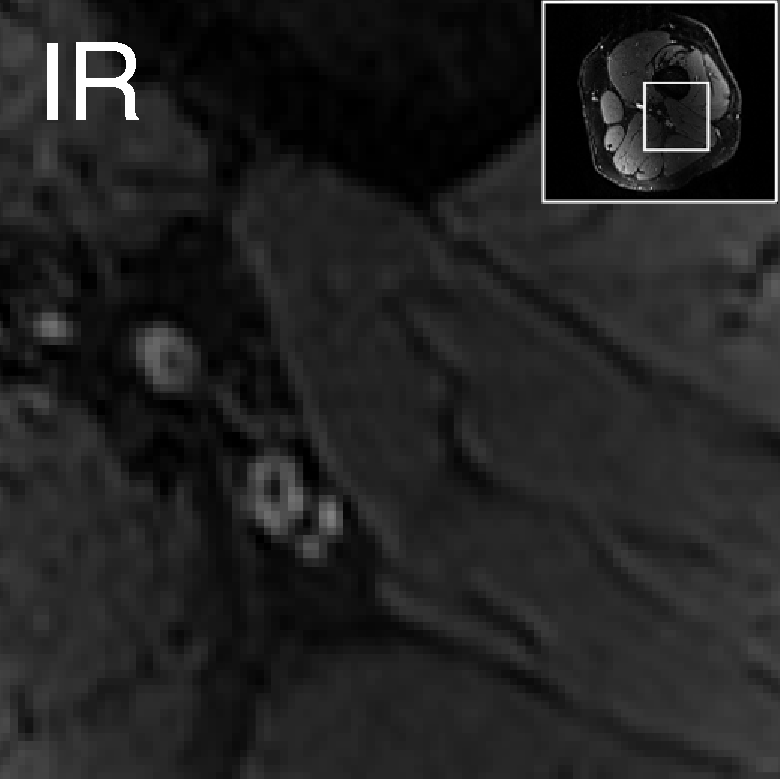
\includegraphics[width=4cm]{channel_IR}
	}
	\hfill
	\subfloat[]
	{
		\label{fig:subfig:T2}
		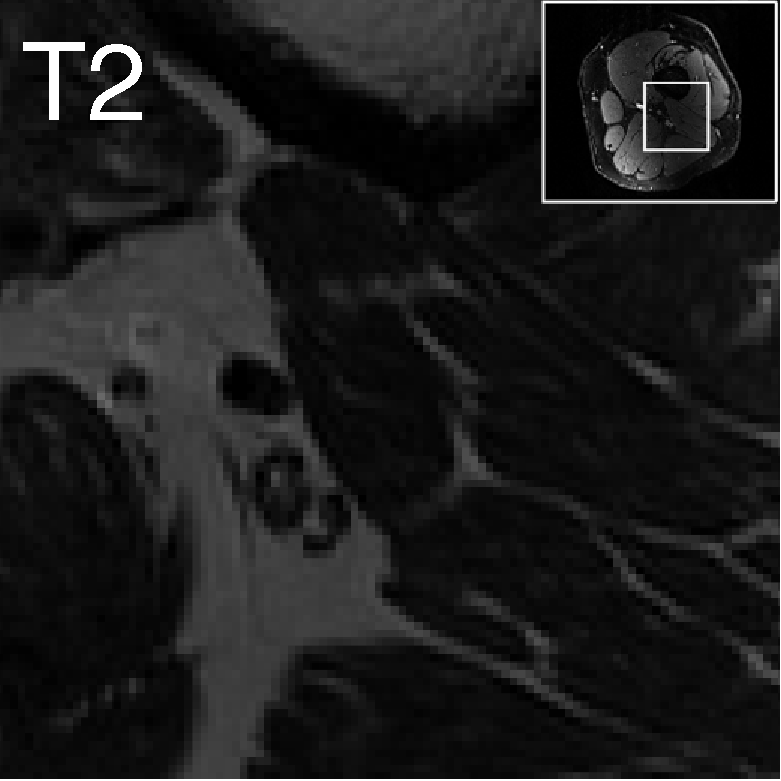
\includegraphics[width=4cm]{channel_T2}
	}
    \hfill
	\subfloat[]
	{
		\label{fig:subfig:GT}
		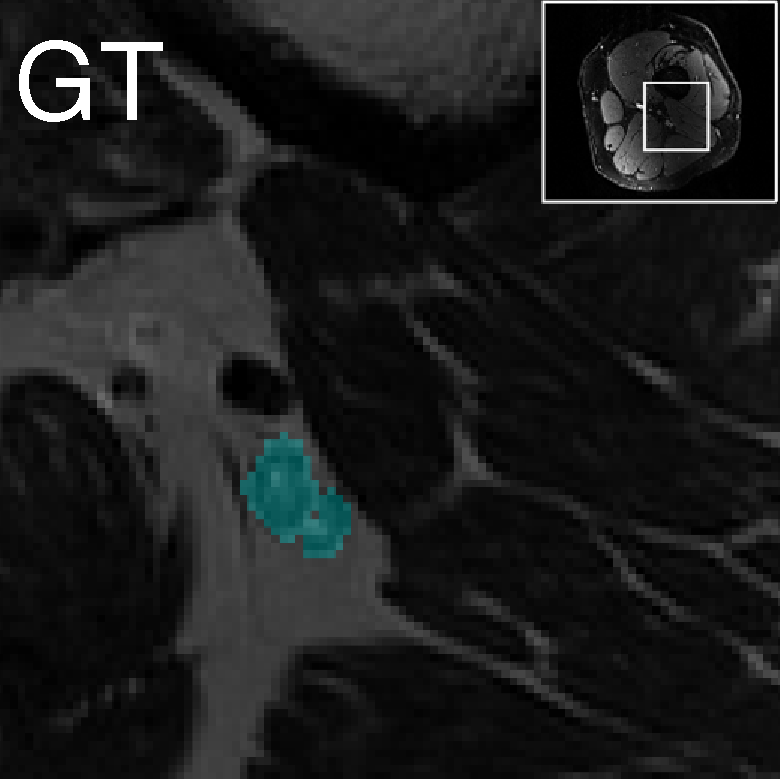
\includegraphics[width=4cm]{channel_GT}
	}
	\caption[Sections of MRN sequences]{Axial image sections of the sciatic nerve proximal to the knee: \textbf{a)} Low-resolution T2-weighted image with fat suppression using \gls{ir}. \textbf{b)} High-resolution T2-weighted image without fat suppression. \textbf{c)} High-resolution T2-weighted image with annotated sciatic nerve. Note that the nerve has a similar appearance as blood vessels in the T2 image.}
	\label{fig:sequences}  
\end{figure}

\subsubsection{Ground Truths} \label{dataset_gt}
For each MRN case, three physicians, experienced in clinical, electrophysiological, and imaging-based assessment of neuromuscular diseases (Olivier Scheidegger (OS), senior neurologist and neuroradiologist > 14 years; Benedikt Wagner (BW), neuroradiologist > 4 years; Lorenz Grunder (LG), neuroradiologist > 2 years) manually segmented the sciatic nerve, including its distal branches the tibial and fibular nerve. The nerve segmentations were performed by each physician individually on the T2-weighted images, allowing the study of the inter-rater agreement. The segmentations were performed with the ITK-SNAP~\cite{py06nimg} software using the polygon or paintbrush tool. The descriptive statistics of the ground truth segmentations are summarized in Table~\ref{tab:ground_truths}. Important to point out is that the number of voxels belonging to the sciatic nerve only account for $0.14 \pm 0.05$ \% of the total image voxels. Figure~\ref{fig:gt_render} shows a 3D-rendering of a sciatic nerve, including the branching, based on the ground truth segmentation of OS.\\
We obtained a consensus ground truth segmentation by the combination of the three expert ground truths via majority voting (GT in Table~\ref{tab:ground_truths}): A voxel was labelled sciatic nerve class if at least two rater segmented it. In our case the obtained consensus ground truth is identical to the result that one would have received by applying the \gls{staple} algorithm~\cite{Warfield2004SimultaneousSTAPLE}, which is a common algorithm for label fusing.\\

\begin{figure}[htbp]
	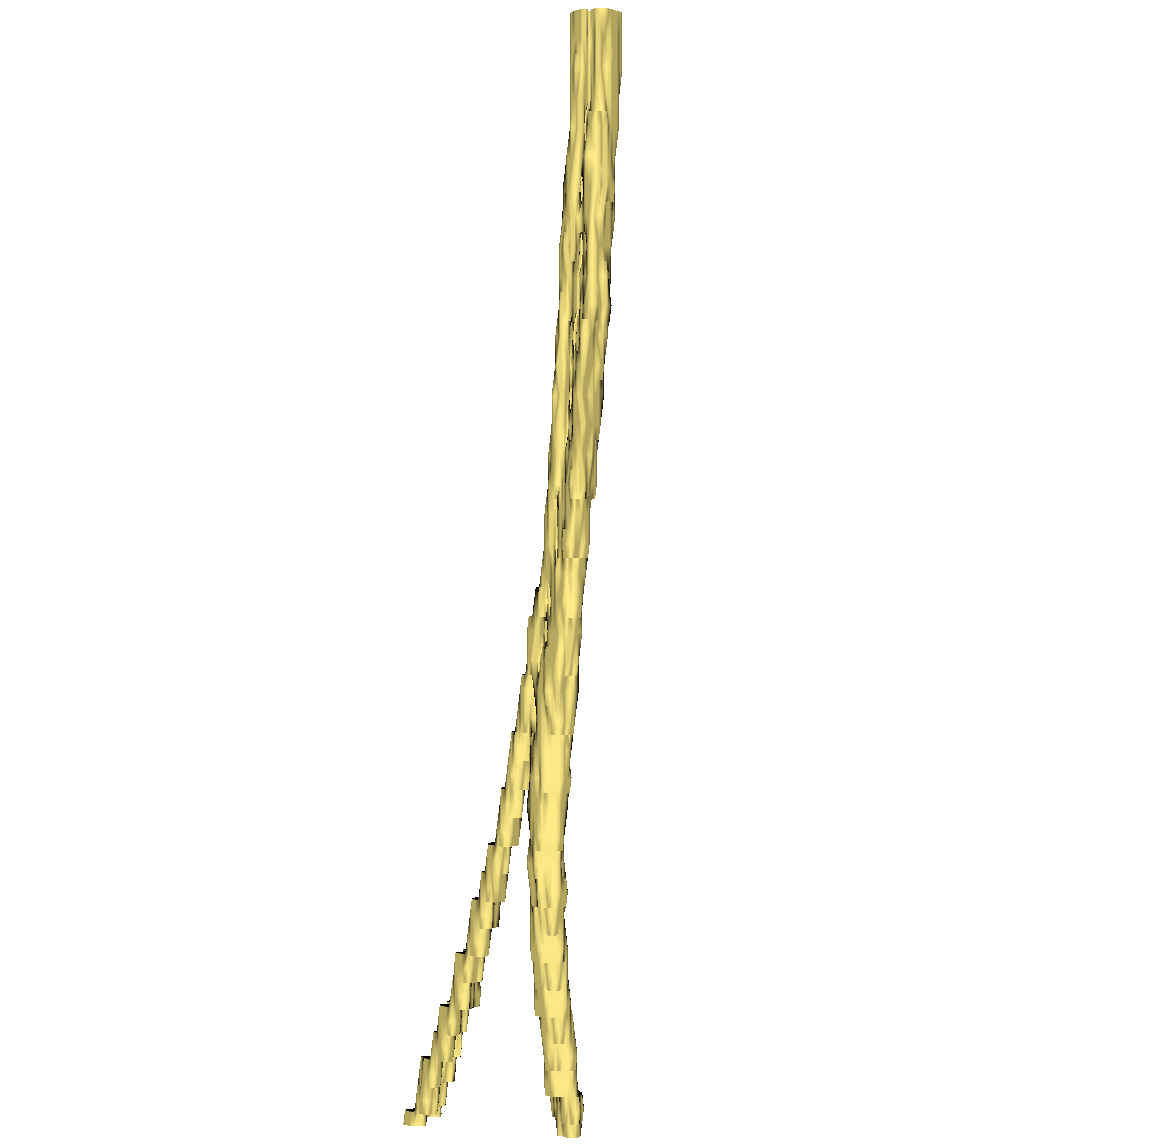
\includegraphics[width=\textwidth]{24A_gt_render}
    \caption[3D-rendering of sciatic nerve]{Anterior view of a 3D-rendering of the sciatic nerve based on the ground truth segmentation (rater OS). Clearly visible is the branching of the sciatic nerve into the tibial and fibular nerve.}
    \label{fig:gt_render}
\end{figure}

\begin{table}[htbp]
   \centering
   \caption[Descriptive statistics of the ground truths]{The segmented ground truths with descriptive statistics of the voxel count and the mean sciatic nerve volume fraction.}
   \begin{tabular}{l*{6}{l}}
      \toprule
      Rater	& Cohort	& Mean		& SD		& Min		& Max		& Mean Volume	\\
      		&			& (voxels)	& (voxels)	& (voxels)	& (voxels)	& Fraction (\%)  \\
      \midrule
      OS  & Patient   & 13373.6 & 4602.1 & 7163.8 & 27428.4 & 0.155 \\
          & Volunteer & 5521.4  & 596.2  & 4615.6 & 6464.4  & 0.103 \\
      BW  & Patient   & 11519.1 & 5086.4 & 3691.7 & 30060.2 & 0.132 \\
          & Volunteer & 4686.8  & 676.1  & 4145.3 & 6299.7  & 0.088 \\
      LG  & Patient   & 12301.8 & 4035.2 & 4613.2 & 22526.4 & 0.142 \\
          & Volunteer & 5375.3  & 674.5  & 4342.2 & 6314.0  & 0.100 \\
      \midrule
	  GT  & Patient   & 11927.2 & 4240.6 & 5860.5 & 24845.5 & 0.138 \\
          & Volunteer & 5145.3  & 612.0  & 4458.0 & 6334.3  & 0.096 \\
      \bottomrule
   \end{tabular}
   \label{tab:ground_truths}
\end{table}


\subsection{Software \& Frameworks}
\subsubsection{Python}
Python\footnote{https://www.python.org/} (Python Software Foundation, Wilmington, DE, U.S.) is an interpreted high-level programming language which is widely used in academia and industry due to its effectiveness. Python is cross-platform and open-source. For all programming in this work we use Python version 3.6 together with (but not exclusively) the packages mentioned below.

\subsubsection{PyTorch}
PyTorch\footnote{https://pytorch.org/} (Facebook, Inc., Menlo Park, CA, U.S.) is a Python package for tensor computations with strong \gls{gpu} acceleration. Although at this point it is officially still in beta state, PyTorch has become an essential framework for deep learning research and applications with a rapidly growing community. We use PyTorch version 0.4.0 to implement and train the neural networks for this work.
\subsubsection{pymia}
The Python package pymia\footnote{https://pymia.readthedocs.io/} is developed and maintained by the \gls{mia} group at the \gls{istb}, University of Bern. The package contains generic and modular code for typical medical image analysis tasks. It offers lots of boilerplate code and we heavily relied on pymia to store, load, and transform the images as well as for the evaluation of the segmentation.
\subsubsection{ITK-SNAP}
ITK-SNAP\footnote{http://www.itksnap.org/} \cite{py06nimg} is an application for inspection and segmentation of medical images. The latest release of ITK-SNAP, version 3.6.0, was used to inspect the \gls{mrn} images, and to render and assess the ground truths and segmentations of the sciatic nerves.
\subsubsection{Seaborn}
Seaborn\footnote{https://seaborn.pydata.org/} is a statistical data visualization package for Python. We used Seaborn version 0.9.0 to analyze and plot our results.
\subsubsection{LibreOffice Calc}
LibreOffice Calc\footnote{https://www.libreoffice.org/} version 6.0.3.2 was used to create spreadsheets for the result tables.

\subsection{Hardware}
Training of the neural networks was done on the \gls{mia} group internal \gls{gpu} server. Most of the networks were trained on an NVIDIA Titan Xp. More demanding experiments, however, were trained on a NVIDIA Quadro P6000. Pre-processing, data augmentation and the calculation of the evaluation metrics were done using the \gls{cpu}. Post-processing was done on a desktop PC with an Intel Core i7 3.2 GHz \gls{cpu}, 64 GB memory and running Ubuntu 16.04 LTS.
\begin{table}[htbp]
   \centering
   \caption{Hardware overview of the \gls{mia} group \gls{gpu} server. \# corresponds to the number of cores or the number available of the respective \gls{gpu} type.}
   \begin{tabular}{l*{3}{r}}
      \toprule
      Property & Hardware & Memory / Frequency & \# \\
      \midrule
      \acrshort{cpu} & Intel Xeon E5-2620 & 2.10 GHz & 32 \\
      \acrshort{ram} & & 64 GB & \\
      GPU & NVIDIA 1080 Ti & 11 GB & 1 \\
       & NVIDIA Titan Xp & 12 GB & 5 \\
       & NVIDIA Quadro P6000 & 24 GB & 1 \\
      \bottomrule
   \end{tabular}
   \label{tab:cluster}
\end{table}

\section{Pre-processing} \label{sec:preprocessing}
Prep-rocessing is only applied to the \gls{mrn} image data of the \gls{ir} and T2 sequences. First, we registered the \gls{ir} image to the T2 image. Second, we normalized the intensities of the \gls{ir} and T2 images.\\
We registered the \gls{ir} image to the T2 image because of its lower in-plane resolution. We used a two step registration: i) rigid registration with three pyramid levels, and ii) affine registration with three pyramid levels. Mutual information~\cite{Maes1997MultimodalityInformation} was used as similarity metric. One setting of registration parameters was tuned for all cases heuristically by qualitative inspection of the registration results.\\
We intensity-normalized the \gls{mrn} images by subtracting the mean of each \gls{mrn} image and dividing by the standard deviation. This results in each \gls{mrn} case having an IR and T2 image with zero mean and unit variance. Input data normalization, as well as normalization in general, can be considered state-of-the-art and have been proven to be beneficial for training and performance of neural networks~\cite{Sola1997ImportanceProblems,SergeyIoffe2015BatchNormalization}.\\
Finally, the images are cropped to the correct input dimensions of the neural network during the data augmentation step, resulting in in-plane dimensions of $300 \times 300$, and $128 \times 128$ pixels respectively.


\section{Segmentation Pipeline}
Our segmentation pipeline has two phases: The training and the evaluation phase, depicted in Figures \ref{fig:pipeline} \textbf{A)} and \textbf{B)}, respectively. We use the pre-processed T2 and IR images together with the ground truth images to train the \gls{fcnn}. The trained \gls{fcnn} can then be used to segment the sciatic nerve from previously unseen (pre-processed) images. Finally, we apply post-processing to further leverage the segmenation accuracy.

The experiments in this thesis focused mainly on the network architectures, and the post-processing. The network architectures are described in Section \ref{sec:architecture} and the post-processing is described in Section~ \ref{sec:postprocessing}. Details to the training are given in the Section \ref{sec:training}.

\begin{figure}[htbp]
	\caption[Segmentation Pipeline]{Overview for the two phases of the whole segmentation pipeline: \textbf{A)} The FCNN is trained with the pre-processed and augmented T2, IR and ground-truth images. The optimizer adjusts the neural networks's weights based on a defined loss function. \textbf{B)} Once fully trained, the FCNN can segment the sciatic nerve on new images without the ground truth image. Finally, optional post-processing is applied.}
	\label{fig:pipeline}
	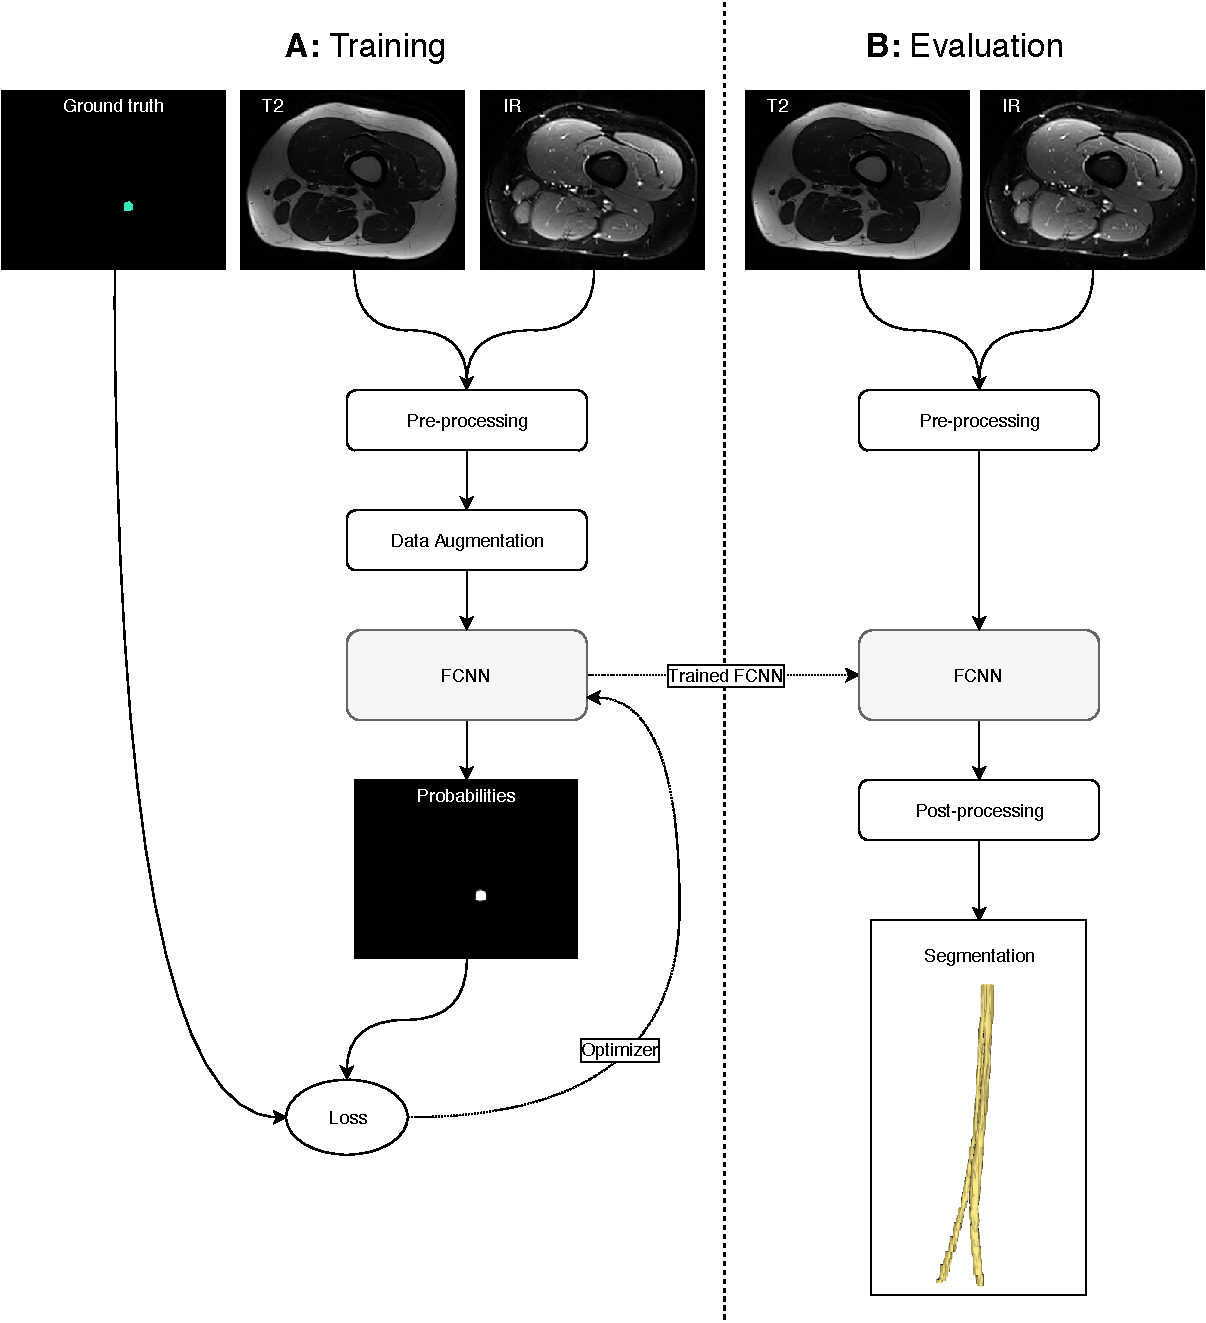
\includegraphics[width=\textwidth]{pipeline}    
\end{figure}

\section{Network Architectures} \label{sec:architecture}
We aim at investigating the optimal architecture and image input format for the segmentation tasks. Therefore, we selected a baseline architecture, which was incrementally changed based on our experiments and observations. As the baseline architecture we selected the U-Net by Ronneberger et al.~\cite{Ronneberger2015U-Net:Segmentation}. The U-Net architecture has proven to work well for semantic segmentation tasks and was originally developed for biomedical image segmentation.

All our \gls{fcnn}'s base on the encoder-decoder architecture of the U-Net, which is depicted in Figure~\ref{fig:unet}. We used a slightly modified version of the original paper based on the current state-of-the-art. We use dropout layers \cite{Srivastava2014Dropout:Overfitting} with probability $p = 0.2$, perform Batch Normalization \cite{SergeyIoffe2015BatchNormalization} and use the \gls{relu} activation function after each convolutional layer for all of our FCNN's. We always perform \textit{same}-padding and a stride of 1 for all convolutions, unless otherwise stated. Additionally we use 32 channels on the first encoder level, doubling the number on each down-transition in the encoder path of the architecture.
Similarly, in the decoder path, we reduce the number of channels by half after each up-transition. We want to segment the images voxels into the two classes \textit{background} and \textit{peripheral nerve}, respectively. This is a binary classification problem. Therefore the out-layer of all our neural networks consists of only one channel. We apply the sigmoid non-linearity to the out-layer to obtain the voxel-wise probability for peripheral nerve.\\
The chosen baseline architecture performs the segmentations on \gls{2d} images. Our \gls{mrn} images, however, are \gls{3d} images and the sciatic nerve is, none-the-less a 3D structure as well. We hypothesize that 3D-contextual information allows a neural network to create better nerve segmentations and therefore a \gls{3d} architecture should perform better than a \gls{2d} architecture. In order to investigate the impact of \gls{3d} information on the segmentation performance, we propose the following three network architectures:
\begin{enumerate}
  \item 2D Baseline
  \item 3D Stack-wise
  \item 3D Patch-wise
\end{enumerate}
The architectures have increasing access to the \gls{3d} information of the sciatic nerve, and are demonstrated in Figure~\ref{fig:inout} with respect to the image dimensions they take as input. The \gls{ir}, T2 and ground truth images are cropped to fit the respective input dimensions. During training phase, the cropping is performed randomly in the plane, as illustrated by Figure~\ref{fig:data_augmentation} and is part of data augmentation which is presented in Section \ref{sec:trainig:data_augmentation}. In the evaluation phase, the segmentations of the \gls{3d} images are performed by splitting the images, predicting and finally merging the prediction maps. These steps are all done based on the input and output dimensions of the respective architecture.

\begin{figure}[htbp]	
	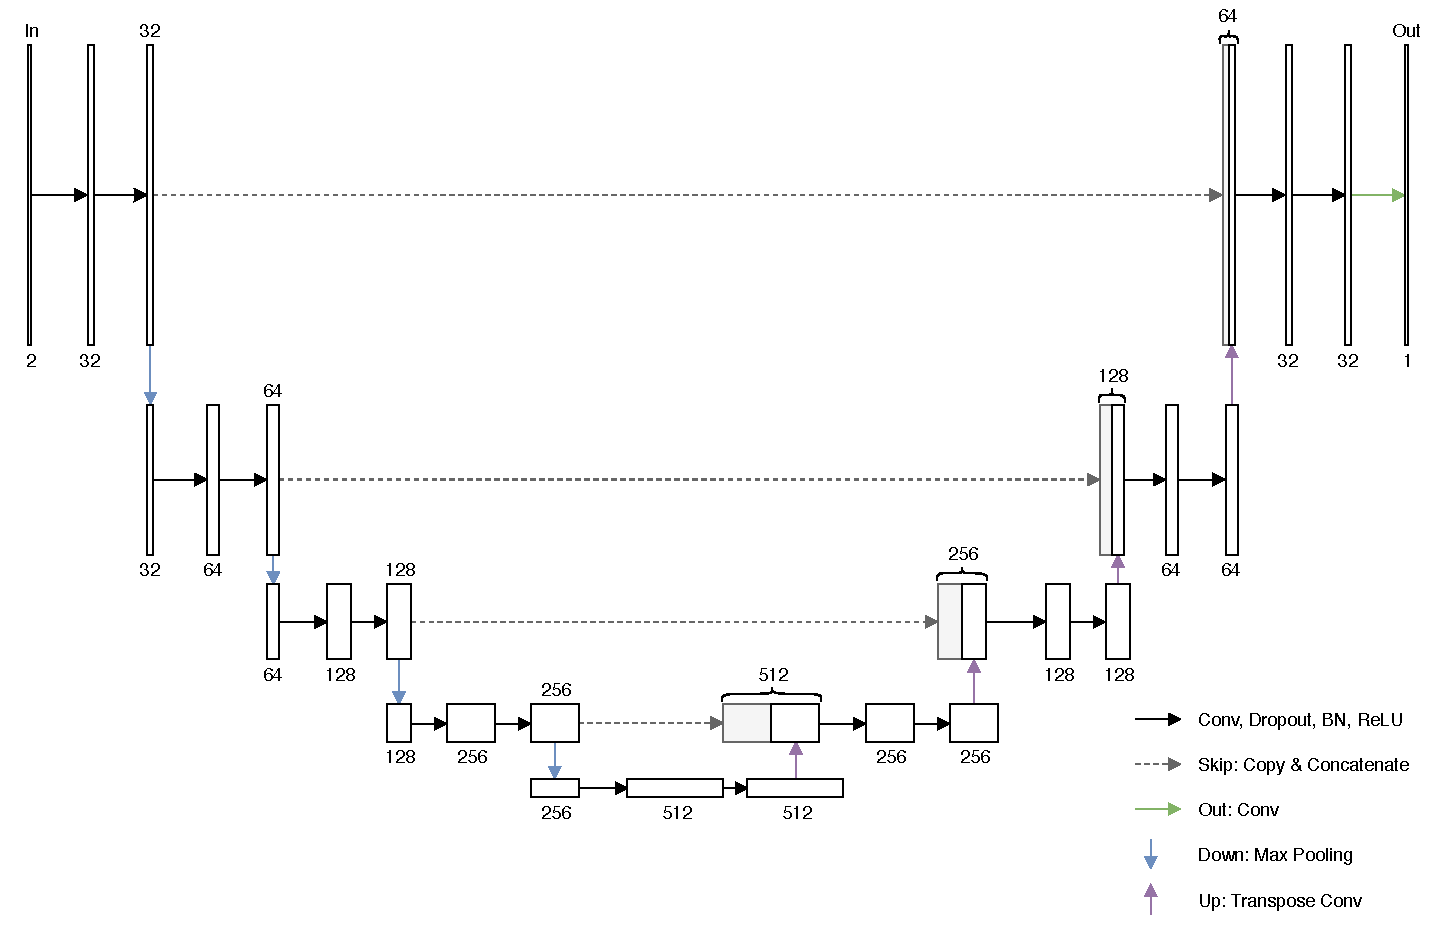
\includegraphics[width=\textwidth]{unet}
    \caption[Network architecture]{The trained \gls{fcnn}s all implement an U-Net-like encoder-decoder architecture. The originally proposed U-Net has been extended by adding a dropout layer and performing \gls{bn} after each convolution layer. The numbers above and below the blocks indicate the number of channels. All convolutions are 3 $\times$ 3.}
    \label{fig:unet}
\end{figure}

\begin{figure}[htbp]
	\centering
	\subfloat[]
	{
		\label{fig:subfig:inout_base}
		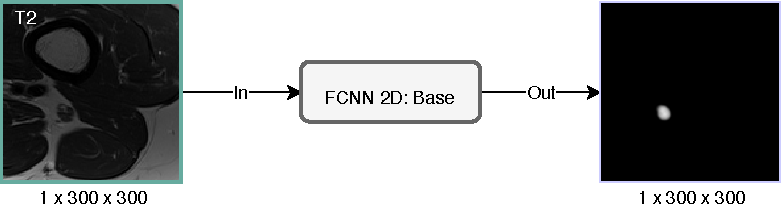
\includegraphics[width=\textwidth]{inout_base}
	}
	\hfill
	\subfloat[]
	{
		\label{fig:subfig:inout_stack}
		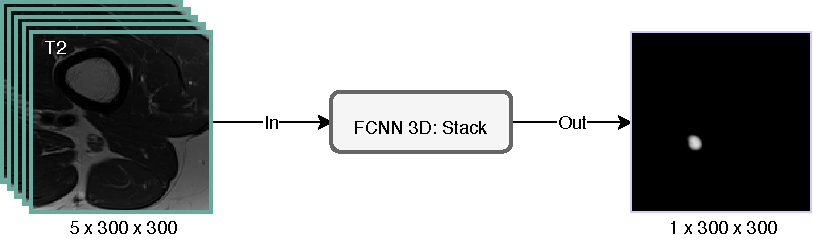
\includegraphics[width=\textwidth]{inout_stack}
	}
    \hfill
	\subfloat[]
	{
		\label{fig:subfig:inout_patch}
		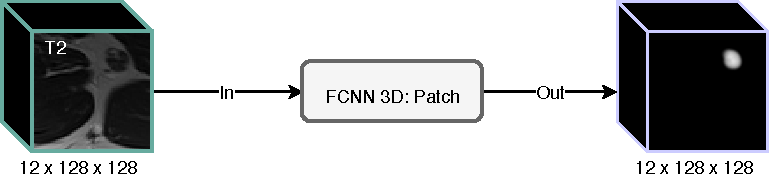
\includegraphics[width=\textwidth]{inout_patch}
	}
	\caption[Inputs and Outputs of the different Architectures]{Depicted are the different input- and output dimensions (in axial, sagittal and coronal direction) for the proposed network architectures. Note, that for simplicity, only the T2 images are shown. The same dimensions apply to the \gls{ir} and ground truth images during the training phase. \textbf{a)} Baseline architecture which takes a single axial slice of $300 \times 300$ pixels as input, and outputs a single slice of probabilities of the same dimensions. The baseline architecture has no access to 3D information of the sciatic nerve at all and therefore is forced to learn \gls{2d} features only. \textbf{b)} The stack architecture receives multiple (5 in the case depicted) slices as input and makes predictions of either 1 or 3 axial slices, depending on the architecture. \textbf{c)} The patch architecture has access to more 3D information (12 slices) along the axial axis, but reduced access in-plane features due to its smaller in-plane resolution. The predictions of this architecture are of the same dimensions as the input.}
	\label{fig:inout}  
\end{figure}

\subsection{2D Baseline}
Our baseline architecture corresponds to the 2D U-Net as proposed by Ronneberger et al. \cite{Ronneberger2015U-Net:Segmentation} with dropout and Batch Normalization added. As mentioned before, we also start with 32 instead of 64 channels on the first encoder level. As Figure \ref{fig:subfig:inout_base} shows, the baseline architecture with its 2D kernels (3x3) handles 2D slices only, and therefore, has no access to 3D-contextual information. The details of the implemented architecture can be found in Table \ref{tab:architecture_fcnn_base} in the appendix.

\subsection{3D Stack-wise}
Driven by our hypothesis, we define an architecture which still closely resembles the baseline architecture, but has more access to the \gls{3d} information in the \gls{mrn} images.
We expand the \gls{2d} U-Net architecture to \gls{3d} by exchanging all building blocks (Convolutional layers, Max Pooling, Batch Normalization) with their \gls{3d} equivalent, similarly to Cicek et al.~\cite{Cicek20163DAnnotation}. In contrast to \cite{Cicek20163DAnnotation}, we keep the number of down- and up-sampling transitions and alternate between 2D kernels ($1 \times 3 \times 3$) and 3D kernels ($3 \times 3 \times 3$) within every level.
We feed this network multiple axial slices of $300 \times 300$ voxels as an input.
With the use of 3D kernels, and the multiple slices as input, the neural network can incorporate more of the 3D information to make predictions.
Details are to be found in in Table~\ref{tab:architecture_fcnn_volumetric} in the appendix. We trained the following versions of this architecture:
\begin{itemize}
  \item 3-to-1: 3 Input slices, prediction of 1 slice.
  \item 5-to-1: 5 Input slices, prediction of 1 slice.
  \item 5-to-3: 5 Input slices, prediction of 3 slices.
\end{itemize}
In essence, we feed the neural network the neighbouring slices (the previous two and next two in case of the 5-to-1 variant) to which it is supposed to make predictions about. We only predict fewer slices than the input slices because we expect to get better segmentation performance. The ability of the neural network to have access to all \gls{3d} information of the neighbouring slices should make it more confident about predictions on the slice(s) in the middle.
For the reason that our \gls{mrn} images have a much higher axial spacing (4.40 mm) as in-plane (0.52 mm) and also a lower axial resolution (30 to 60 slices) we decide to keep the up- and down-transitions in-plane and therefore do not perform pooling along the axial axis.\\
As test, and to further investigate the impact of \gls{3d} information we decided to train the 5-to-3 architecture and additional time with a experimental loss function based on projections: Instead


\subsection{3D Patch-wise}
We increase the accessible 3D information along the axial axis even further by defining a network architecture similar to Cicek et al.~\cite{Cicek20163DAnnotation} featuring one up- and down-transition less than the other architectures. We conducted an experiment where we feeded the \gls{mrn} images to the neural network. We, however, were unable to successfully train the neural network and therefore decided to continue with a patch-based approach: We decrease the in-plane input dimensions to $128 \times 128$, and therefore reduce the accessible in-plane information for the network. We increase the number of slices fed to the network to 12. Furthermore the up- and down-transitions are only applied in the in-plane dimensions for the same reasons as mentioned for the stack-wise architecture. All the convolutional layers feature 3D kernels ($3 \times 3 \times 3$). The exact architecture is listed in table \ref{tab:architecture_fcnn_patches}.

\section{Training} \label{sec:training}
This section describes how we trained our neural networks and, therefore, corresponds to the steps depicted in Figure~\ref{fig:pipeline} \textbf{A)}. Once trained, a neural network is evaluated according to Section~\ref{sec:evaluation} and depicted in Figure~\ref{fig:pipeline} \textbf{B)}.

\subsection{Data Augmentation} \label{sec:trainig:data_augmentation}
A common problem during the training of neural networks is called overfitting. During training, the weights of the neural network get adjusted via the optimizer to reduce the loss on the training set. The primary goal of the training is to emphasize the neural network to learn meaningful features which generalize to previously unseen data, which is typically defined by the test set. 
Depending on the capacity of the neural network (its ability to fit a wide variety of functions, i.e. data \cite{Goodfellow2016DeepLearning}), the complexity of the task to solve, and the size of the training set, a neural network can start to overfit. If the neural network is somewhat complex, and training data is sparse, the neural network can begin to memorize the training examples rather than learning important features. This results in a high test-loss and hence a low performance on previously seen data, despite the training-loss being very low. Several counter-measures to overfitting exist, of which the most effective one is merely to use a bigger dataset. However, gathering and preparing a bigger dataset is time-consuming and often not possible, especially for medical images.\\
A possibility is to re-train the network in its capacity by reducing the numbers of convolutional layers or the number of features per convolutional layer.
Furthermore, there exist a variety of regularization techniques which may help:
$L^2$ (weight decay), $L^1$ (sparsity), early stopping \cite{Goodfellow2016DeepLearning}, dropout \cite{Srivastava2014Dropout:Overfitting}, and others.\\
One way to get around the problem of little annotated data is to create fake data and add it to the training set. This practice is known as data augmentation. Depending on the problem, the augmented data can be obtained either through transformation (e.g., cropping, flipping, mirroring, rotating) of existing training examples or can also be generated fully synthetically \cite{Tetteh2018DeepVesselNet:Volumes}.\\
We applied data augmentation by randomly transforming the data online during the training phase of the neural networks. We tested different sequences of transformations, including random crops, rotations, mirroring, elastic transformations and mixup, as proposed by Zhang et al.~\cite{Zhang2017Mixup:Minimization}, to prevent overfitting. In contrast to Eaton-Rosen et al.~\cite{Eaton-rosen2018ImprovingSegmentation}, mixup did not improve training or performance of the neural networks for us. The same was the case with the elastic distortions, so we decided not to use them. Figure \ref{fig:data_augmentation} shows the sequence of random transformation applied to each training sample before it was fed to the neural network during training: First, we randomly crop the input images (IR and T2) and the ground truth to the in-plane dimensions of $300 \times 300$ pixels. Second, we rotate the cropped images in-plane between 0 to 3 times randomly by 90\si{\degree}. Last, we mirror the images along the vertical edge in half of the cases.

\begin{figure}[htbp]	
	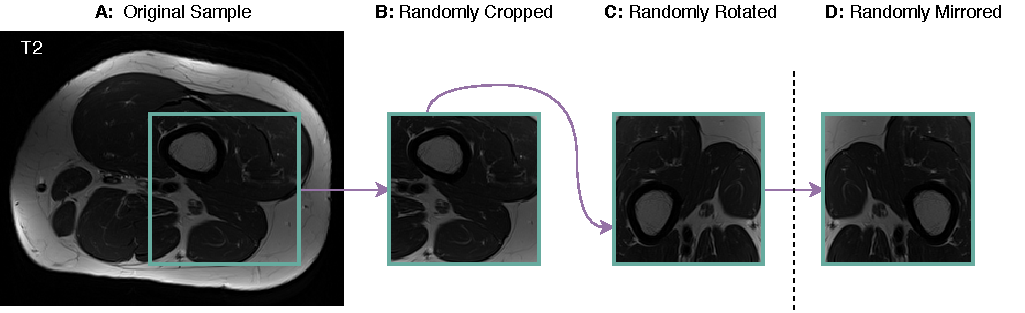
\includegraphics[width=\textwidth]{data_augmentation}
    \caption[Data Augmentation]{The sequence of random transformations applied to each training sample before feeding it to the neural network: \textbf{A)} The T2 image  before the data augmentation. \textbf{B)} Random crop to the dimensions $300 \times 300$. \textbf{C)} Rotation into a random direction. \textbf{D)} Mirroring with 50~\% probability. Note that the same transformation (per training sample) is applied to T2 image, IR image and ground truth, respectively. Furthermore, we also apply the same transformation to each slice for the neural networks which take multiple slices as input. }
    \label{fig:data_augmentation}
\end{figure}

\subsection{Loss Function}
We used the binary cross-entropy loss to train our neural networks. Due to the small amount of voxels belonging to the sciatic nerve (0.14\%) the segmentation task results in a highly imbalanced classification problem, with the \textit{background}-class, i.e. no sciatic nerve, being over 99 times more abundant than the \textit{sciatic-nerve}-class. This makes the training of the neural networks heavily biased towards background segmentation: In the beginning, the training loss can easily be reduced substantially by assigning all voxels to the \textit{background}-class. This is a common problem for medical image segmentation tasks with neural networks~\cite{Litjens2017AAnalysis,Tetteh2018DeepVesselNet:Volumes,Baumgartner2017AnSegmentation,Selvan2018ExtractionNetworks,Kayalibay2017CNN-basedData}\\
Buda et al.~\cite{BudaANetworks} systematically analyzed the impact of class imbalance on the classification performance on \acrshort{cnn}'s. They list and compare frequently applied solutions to this issue.\\
A solution to class imbalance is to use a weighted- or rebalancing loss. Ronneberger et al. \cite{Ronneberger2015U-Net:Segmentation} and Cicek et al.~\cite{Cicek20163DAnnotation} use a weighted cross-entropy loss to train their 2D and 3D U-Nets, respectively. Milletari et al.~\cite{Milletari2016V-Net:Segmentation} introduced a loss based on the Dice similarity coefficient, to account for the class imbalance. Several works, especially in the medical domain, successfully applied this loss or a variant of it \cite{Selvan2018ExtractionNetworks,Kayalibay2017CNN-basedData,Drozdzal2016TheSegmentation}. Sudre et al.~\cite{Sudre2017GeneralisedSegmentations} investigated the behaviour of weighted cross-entropy, sensitivity and Dice losses for their sensitivity to different rates of class imbalance in 2D and 3D segmentation tasks. They concluded that, depending on the imbalance rate, the use of the weighted or rebalancing losses help the optimization. Baumgartner et al.~\cite{Baumgartner2017AnSegmentation} compared cross-entropy, weighted cross-entropy and the Dice loss on different network architectures for cardiac MR image segmentation. They achieved superior performances with the cross-entropy losses (the weighted version being marginally better) and concluded, that for their task, the class imbalance was not a problem. They, however, reported a foreground prevalence of approximately 25\% which is significantly higher than our prevalence of 0.14\%.\\
Based on these results we conducted experiments with the baseline architecture to evaluate the benefit of weighted cross-entropy and Dice loss. Conversely to the results, we did not see any improvements during training or in the final performance when compared to unweighted cross-entropy loss. We, therefore, decided to use the binary cross-entropy loss for all our experiments. Additionally, we calculated and used the \acrlong{dice} in conjunction with the training and test losses to monitor the training progress.

\subsection{Optimizer}
We use PyTorch's implementation of the Adam optimizer \cite{Kingma2014Adam:Optimization} without weight decay, $\beta_1 = 0.900$, and $\beta_2 = 0.999$ for the training of all networks. A listing of all hyperparameters can be found in Table~\ref{tab:hyperparameters} in the appendix.

\section{Post-processing} \label{sec:postprocessing}
\begin{figure}[htbp]
    \centering
	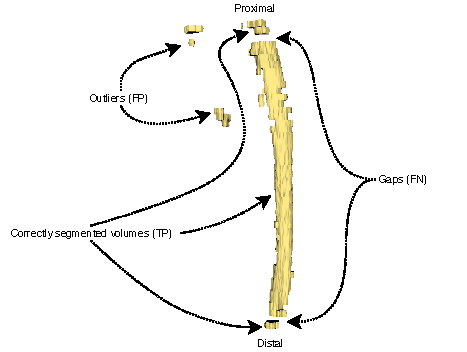
\includegraphics[width=\textwidth]{fpfn}
    \caption[Issues of the Segmentations]{First results showed that the unprocessed segmentations were typically corrupted by false positive (FP) outliers and false negatives visible as gaps. While the outliers impact the distance metrics, i.e. \gls{hd}, the gaps make post-processing harder: Simply keeping the largest volume present, would remove all smaller correctly segmented volumes (TP).}
    \label{fig:fpfn}
\end{figure}
Early experiments showed that there are \gls{fp} outliers as well as \gls{fn} discontinuities present in the segmentations, see Figure~\ref{fig:post_processing}. The distance metrics, especially the \acrshort{hd}, are sensitive to these (\acrshort{fp}). The (\acrshort{fp}) outliers all tend to have small volumes and therefore could easily be removed by keeping only the largest volume present in the segmentation. The presence of (\acrshort{fn}), visible as gaps, however, makes this a more difficult task: They split the nerve into multiple correctly segmented volumes (\acrshort{tp}). Simple and naive post-processing by keeping only the largest volume, would also remove all smaller correctly segmented volumes.\\
With the aim to increase the quality of sciatic nerve segmentations by reducing the (\acrshort{fp}), we apply the two following post-processing steps to the output of a neural network: First, we try to connect the correctly segmented volumes to form one large volume. Second, we only keep the largest volume.\\
\begin{figure}[htbp]	
	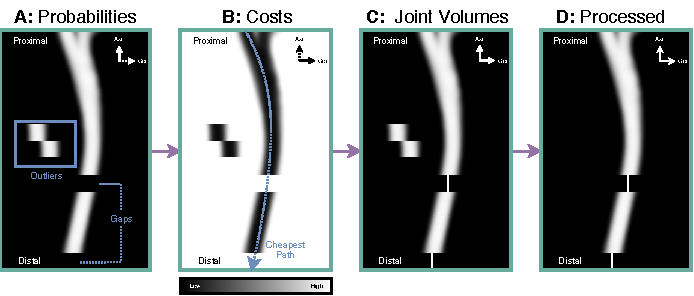
\includegraphics[width=\textwidth]{post_processing}
    \caption[Steps of Post-processing]{Post-processing steps applied ot the output of a neural network to increase segmentation performance. \textbf{A)} Output of the neural network corrupted by outliers (FP) and gaps (FN). \textbf{B)} Costs for the calculation of the cheapest path. Costs are obtained by taking the background probabilities ($p_{background} = 1 - p_{nerve}$) for each voxel. Cheapest path is along the (TP) volumes. \textbf{C)} All voxels along the cheapest path are labelled as nerve, merging the (TP) volumes to one big volume. \textbf{D)} All but the biggest volume are removed, resulting in fewer (FP).}
    \label{fig:post_processing}
\end{figure}
Given the anatomy of the sciatic nerve and the anatomical region the MRN images were taken from, we know it passes through both, the most proximal and distal slice. Additionally, we know that all (\acrshort{tp}) lie on a long tubular-like path along the cario-caudal axis given by the anatomy of the sciatic nerve. Once we know the path, we can use it to connect the (\acrshort{tp}) volumes.\\
We treat this as a directed graph problem, where we want to find the cheapest path from the most proximal to the most distal slice. The intermediate steps are depicted in Figure~\ref{fig:post_processing}: \textbf{A)} The predictions of the neural networks can be corrupted by (\acrshort{fp}) and (\acrshort{fn}). \textbf{B)} Therefore, we define the voxels of the probability image to be the graph nodes, with each having a cost of the inverse of the sciatic nerve probability to pass through. Therefore, voxels with high probability being peripehral nerve are cheap and hence favourable candidates to be part of the cheapest path. To find the cheapest path through the graph we make use of Dijkstra's Algorithm~\cite{Dijkstra1959AGraphs}. \textbf{C)} Once the cheapest path is found, we label all voxels on the path to belong to the sciatic nerve. This step joins all TP volumes on the path to form one large connected component. \textbf{D)} After we merged all TP to one volume, we only keep the largest component/volume.

\section{Evaluation} \label{sec:evaluation}
This section describes how we evaluate our neural networks after the training phase. Section~\ref{sec:eval_cross} explains the evaluation scheme we apply. In Section~\ref{sec:eval_metrics} our evaluation metrics are presented and Section~\ref{sec:eval_strategy} describes how we deal with the fact that our neural networks have other input dimensions than the dimensions of our \gls{mrn} images.

\subsection{Cross-validation} \label{sec:eval_cross}
In deep learning, evaluation of a model is typically done by \gls{lpocv}: $p$ samples are left out from the dataset to form a training set and validation set of sizes $|S_{train}| = n - p$ and $|S_{valid}| = p$, respectively. As the name implies, the model is trained on the training set. The validation set is used to validate and tune the hyperparameters of the model.
Depending on the dataset size, the split is done randomly or in a semi-random fashion to ensure that the subsets have the same distribution of samples.
A good practice is to split the dataset in the same manner into three subsets, namely the training, validation and test set. Typical values for the split fractions could be 0.7, 0.1 and 0.2 for training-, validation- and test-set respectively. As no data of the test set is used for training or tuning the model, the test set allows evaluating the metrics (Section~\ref{sec:eval_metrics}) on unseen data. \\
The split of the dataset into three separate subsets with similar sample distribution is, however, not always possible, especially if dataset sizes are small. In such cases, evaluation with a \gls{kfcv} may be more a more practical choice: The dataset is split into $k$ equal sized folds, still aiming to have similar sample distributions. Sequentially, one of the folds is left out and used as a validation set, while the model is trained on all of the remaining folds. An approximate accuracy and performance on unseen data can be obtained by averaging the results of the evaluation metrics calculated on the $k$ validation folds.\\
As the size of our dataset (n = 52) is comparably small to other datasets we chose to validate our models via four-fold cross-validation, i.e. our models are trained on 39 subjects and evaluated on 13 subjects. We randomly assigned the patient subjects to the folds but with stratification regarding the volunteers. I.e. we ensured that the volunteers are equally distributed. The assignment of the subjects is summarized in the Table \ref{tab:fold_assignment}. We trained and tuned the neural networks only using the reported semi-random assignment. We did not use any other assignment to develop the method.

\subsection{Metrics} \label{sec:eval_metrics}
To measure and assess the performance of a neural network, evaluation metrics are required. The metrics are calculated by comparison of the segmentation mask (the output of a neural network) to the ground truth obtained by majority voting of the manual expert segmenations. Taha and Hanbury~\cite{Taha2015MetricsTool} analyzed popular metrics for 3D medical image segmentation and provided metric selection guidelines. Based on the guidelines, we choose the following evaluation metrics, and report their mean and \gls{sd} in Chapter~\ref{chap:results}.

\begin{itemize}
\item \acrlong{dice}:
  \begin{itemize}
  \item Outliers are to be expected.
  \item De-facto gold standard.
  \end{itemize}
\item \acrlong{vs}
  \begin{itemize}
  \item Good nerve volume agreement is of clinical interest.
  \end{itemize}
\item \acrlong{avd}
  \begin{itemize}
  \item Sciatic nerve segmentations satisfy conditions for small segments.
  \item Low sensitivity to outliers.
  \end{itemize}
\item \acrlong{hd95}
  \begin{itemize}
  \item Sciatic nerve segmentations satisfy conditions for small segments.
  \item Low sensitivity to outliers
  \item Comparison to publications.
  \end{itemize}
\item \acrlong{hd}
  \begin{itemize}
  \item Sciatic nerve segmentations satisfy conditions for small segments.
  \item We want to analyze the impact of our Post-processing
  \item Comparison to publications.
  \end{itemize}
\end{itemize}

Let $S \in \{0, 1\}$ be the output segmentation mask of a model and $G \in \{0, 1\}$ be the ground truth.
$S_{1}$ denotes the set of all voxels where $S = 1$, i.e., where the neural network detected the foreground. Analogously, $G_{1}$ denotes the set of all voxels where $G = 1$. The number of all voxels in a set $A$ is denoted by the cardinality operator $|A|$.

\subsubsection{\acrlong{dice}}
The \gls{dice} \cite{Dice1945MeasuresTh} is an overlap metric defined as the following:
\begin{equation}
   DICE(S, G) \in [0, 1] = \frac{2|S_{1} \cap G_{1}|}{|S_{1}| + |G_{1}|}.
   \label{eq:dice}
\end{equation}
The \gls{dice} is the most used metric for validating medical image segmentations \cite{Taha2015MetricsTool}. A \gls{dice} value of $1.0$ corresponds to a perfect volumetric overlap of the neural networks foreground segmentation and the ground truth. Important to mention is that the significance of the \gls{dice} drops with increasing volume fraction of the foreground. For instance, a ground truth with a foreground volume fraction of 50\% and a randomly initialized segmentation mask lead to a \gls{dice} of $0.5$. Consequently, the \gls{dice} is much more meaningful in the case of a low volume fraction of the foreground. The fact that the sciatic nerve only accounts for about 0.14\% of the voxels makes this metric well suited for our problem. This, however, means also that we are generally obtaining lower \gls{dice} coefficients which has to be considered when we make comparisons to other segmentation problems with higher foreground prevalence.

\subsubsection{\acrlong{vs}}
The \gls{vs} \cite{Taha2015MetricsTool} is, as the name implies, a volume-based metric. The \gls{vs} can be defined in terms of the \gls{vd} as $1 - \acrshort{vd}$. That is
\begin{equation}
   VS(S, G) \in [0, 1] = 1 - \frac{||S_{1}| - |G_{1}||}{|S_{1}| + |G_{1}|}.
   \label{eq:vs}
\end{equation}
As \gls{vs} is only considering the volumes, the metric does not allow any inference on the alignment or agreement of the shapes of the compared segmentations. This means two segmentations with no overlap at all, consequently with a \gls{dice} of zero, can still result in a high \gls{vs} or even have the same VS, i.e. a VS of 1. In contrary, a high \gls{dice} will always result in a high \gls{vs} because the \gls{vs} is directly correlated to the \gls{dice}.

\subsubsection{\acrlong{hd}}
The \gls{hd} is a distance metric between two sets $S$ and $G$ defined by
\begin{equation}
   HD(S, G) = \max(d_{H}(S,G),d_{H}(G,S)),
   \label{eq:hd}
\end{equation}
where $d_{H}(S,G)$ is the directed \gls{hd} that is given by
\begin{equation}
   d_{H}(S, G) = \max\limits_{s \in S} \min\limits_{g \in G} ||s-g||,
   \label{eq:dhd}
\end{equation}
where $||s-g||$ is some norm, e.g. the Euclidean distance. The \gls{hd} is generally susceptible to outliers, which we have present in the outputs of the neural networks in form of false-positively segmented regions. It is therefore not recommended to directly use the \acrshort{hd} \cite{Taha2015MetricsTool}. Instead, Huttenlocher et al. \cite{Huttenlocher1993ComparingDistance} proposed to use the \gls{hd95}, which is less outlier sensitive. We will report both, \gls{hd} and the \gls{hd95} to be able to compare the metrics.

\subsubsection{\acrlong{avd}}
The \gls{avd}, also known as the average \gls{hd}, is the \gls{hd} averaged over all distances. It is stable and less sensitive to outliers when compared to the \gls{hd}, and also less sensitive than the HD95~\cite{Taha2015MetricsTool}. The \gls{avd} is defined by
\begin{equation}
   AVD(S, G) = \max(d_{AH}(S,G),d_{AH}(G,S)),
   \label{eq:avd}
\end{equation}
where $d_{AH}(S,G)$ is the directed average \gls{hd} that is given by
\begin{equation}
   d_{AH}(S, G) = \frac{1}{N} \sum\limits_{s \in S} \min\limits_{g \in G} ||s-g||.
   \label{eq:dahd}
\end{equation}

\subsection{Strategy} \label{sec:eval_strategy}
Our neural networks have smaller input dimensions than the typical size of the \gls{mrn} images ($60 \times 330 \times 384$). We need, therefore, to split the \gls{mrn} images into junks of the respective input dimensions during the evaluation phase. The junks are then fed sequentially to the neural network, and the obtained probability maps are combined to form a segmentation of the whole volume. We do the splitting and combination slice-wise for the baseline and stack-wise architectures. We crop the slices centrally to an in-plane resolution of $300 \times 300$ voxels to fit the input dimensions of the architectures. The sciatic nerves, generally located central in the transverse plane, lie within the cropped images. No cropping is needed in the case of the patch-wise architecture: The whole image is split into $12 \times 128 \times 128$ volume patches, predicted, and recombined to form the segmentation. The process of dividing, predicting and combining the \gls{mrn} images is explained in Figure~\ref{fig:eval_strategy} in more detail.

\begin{figure}[htbp]
	\centering
	\subfloat[]
	{
		\label{fig:subfig:eval_stack}
		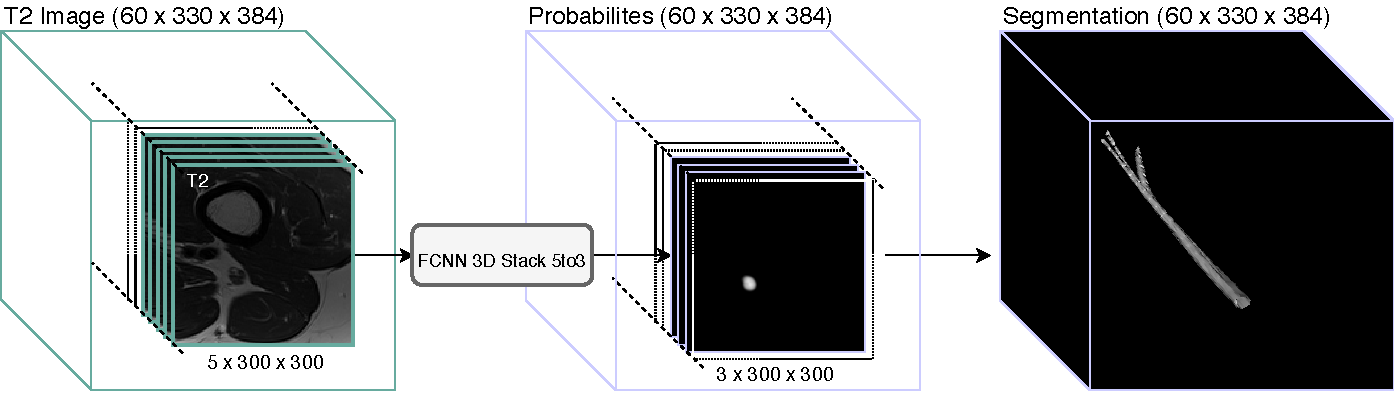
\includegraphics[width=\textwidth]{eval_stack}
	}
	\hfill
	\subfloat[]
	{
		\label{fig:subfig:eval_patch}
		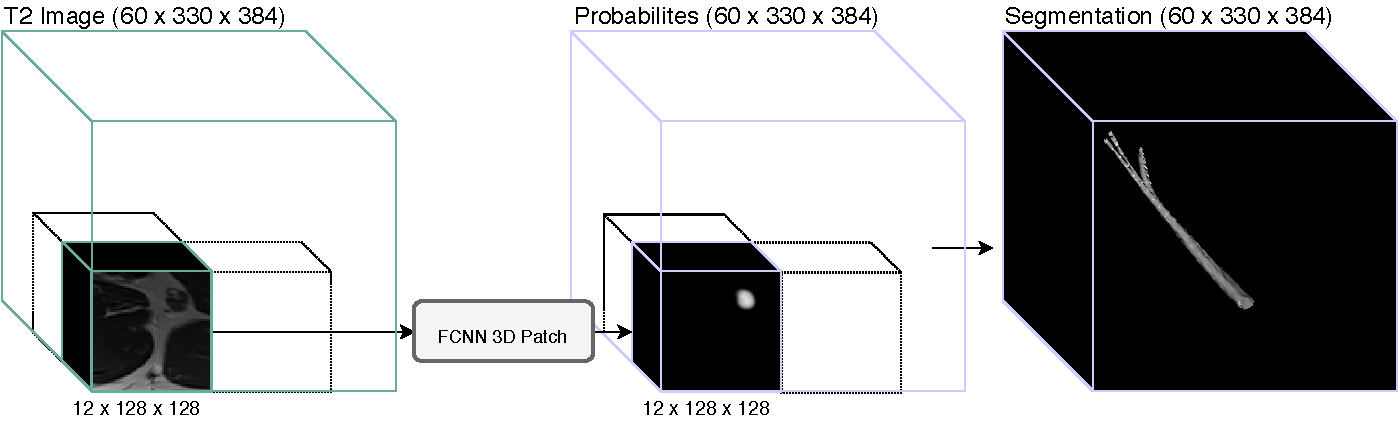
\includegraphics[width=\textwidth]{eval_patch}
	}
	\caption[Evaluation Strategy]{In the evaluation phase, a segmentation with the same dimensions as the ground truth is required from the trained neural network. In order to obtain the segmentation, the image is split into (stacks of) slices or volumes and fed to the neural network. The probability maps, which are the output of the network, are stitched together yielding a probability map of the whole volume. Simple thresholding of the probabilities results in the segmentation, which in return is used to calculate the evaluation metrics upon, together with the ground truth. \textbf{a)} The evaluation for the baseline and stack-wise architectures is done slice-wise: All slices are cropped centrally to an in-plane resolution of $300 \times 300$ voxels and fed sequentially to the neural network (in blocks of 3 or 5 for the stack-wise architecture). The resulting probability maps are concatenated, thresholded and symmetrically padded back up to the input/ground truth dimensions \textbf{b)} To get the segmentation of the patch-architecture, the input image is split into multiple $12 \times 128 \times 128$ patches. The patches are fed to the network sequentially yielding probability patches. These are combined and thresholded to obtain the segmentation.}
	\label{fig:eval_strategy}  
\end{figure}


\section{Experiments} \label{sec:experiments}
We propose the following experiments to validate our hypothesis:\\

\textit{Experiment 1:} We train and evaluate the baseline architecture on our \gls{mrn} images to investigate whether a deep learning-based approach for fully-automatic peripheral nerve segmentation is feasible.

\textit{Experiment 2:} Driven by the hypothesis that \gls{3d} context allows for better segmentation results, we train and evaluate the stack-wise and patch-wise architectures on our \gls{mrn} images and compare their performance to the segmentation performance of the baseline architecture. We do not apply post-processing.

\textit{Experiment 3:} We take our best performing architecture and compare the segmentation performance with and without post-processing applied.

Finally, for evaluation, we take the best performing combination of architecture and post-processing of the experiments and compare the performance to the inter-rater variability.

\endinput